\documentclass[11pt,a4paper]{article}
\usepackage[utf8]{inputenc}
\usepackage[spanish]{babel}
\usepackage{biblatex}
\usepackage{amssymb, amsmath, amsbsy}
\usepackage{graphicx}
\usepackage{makeidx}
\usepackage{color,xcolor}
\usepackage[left=2cm,right=2cm,top=2cm,bottom=2cm]{geometry}
\usepackage[linkcolor=black,colorlinks=true,urlcolor=blue]{hyperref}
\usepackage{xcolor}
\usepackage{fancyhdr}
\usepackage{float}
\usepackage{subfigure}
\renewcommand{\baselinestretch}{1.5}
\addbibresource{bib.bib}
\setlength{\parindent}{0em}
\bibliography{bib}

\begin{document}

\thispagestyle{empty}
\begin{center}

\includegraphics[width=10cm]{logo udesa.PNG}
\end{center}


	\begin{center}
	\LARGE
	Herramientas Computaciones para Investigación
\\			\vspace{1cm}
\hrule
	\vspace{0.5cm}
	\LARGE
 Tema 4 - Data Visualization
\\		
		\vspace{0.5cm}
		\hrule
				\vspace{1cm}
	\large

	\vspace{2.5cm}
	\large
		Alumnos:\\
	\large
	Elard Amaya, Francisco Guerrero
	
	
	\vspace{1.3cm}
	\normalsize	
	Profesora:\\

	\normalsize
	Amelia Gibbons
	
	\vspace{1.3cm}
	\today
	\end{center}

\clearpage
\section{Gráfico 1 - Correlación entre consumo eléctrico y PBI por país}

\begin{figure}[!h]
    \centering
    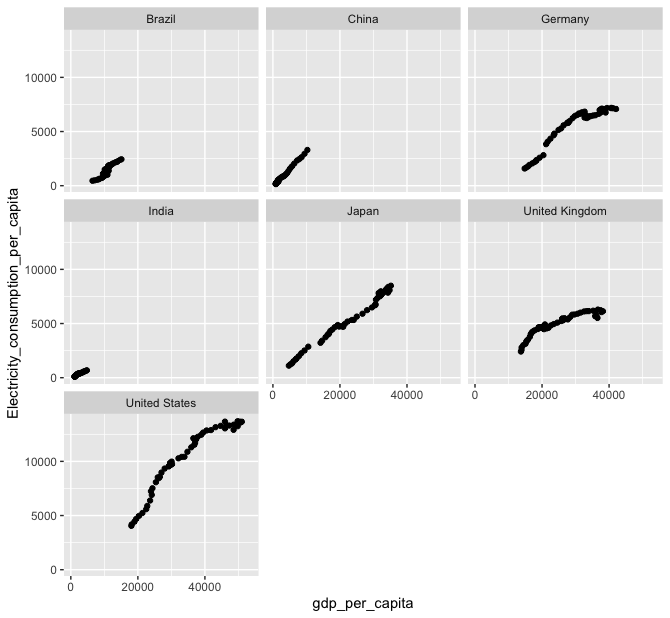
\includegraphics[width=9cm]{old/graph1.png}
\end{figure}

\begin{figure}[!h]
    \centering
    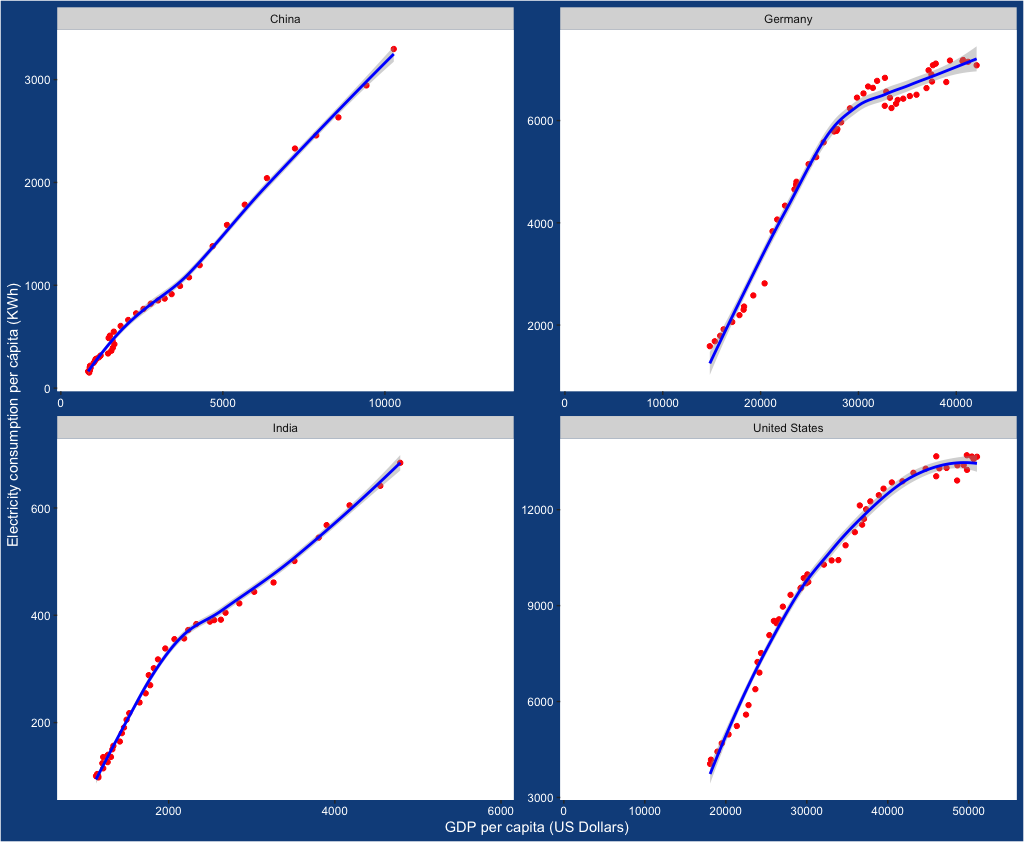
\includegraphics[width=12cm]{new/graph1.png}
\end{figure}

Entre los principales cambios que hemos realizado se encuentran la reducción de los países incluidos en el gráfico, el cambio del fondo a uno azul marino, el cambio de las etiquetas de los ejes y la liberación de la escala de los ejes para que cada uno se vea respecto a su máximo relativo. Tal vez el cambio más importante que realizamos fue añadir una línea de proyección polinómica, la cual nos permite observar si los países estan consumiendo eficientemente su energía eléctrica a medida que aumenta el PBI. Por ejemplo, Alemania es un país con alto nivel de PBI per-cápita y que consume un nivel relativamente bajo de de energía electrica, en comparación con países del mismo nivel de PBI.

\clearpage
\section{Gráfico 2 - Ingreso neto por estudio y género de película}

\begin{figure}[!h]
    \centering
    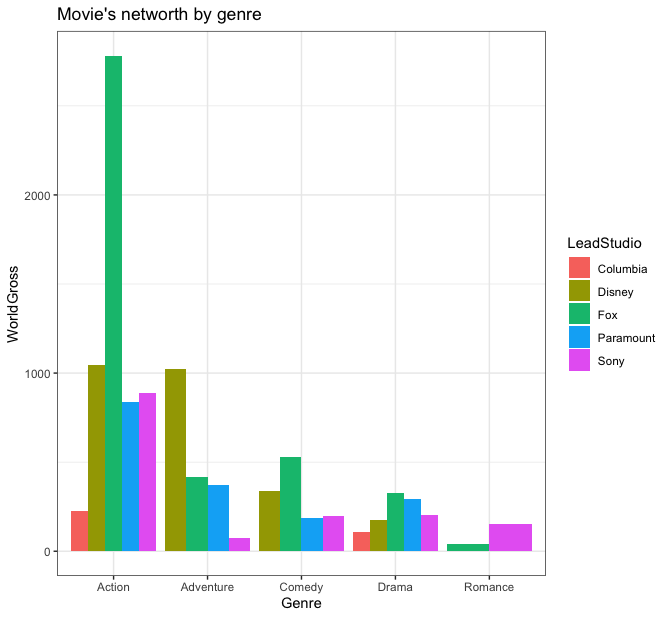
\includegraphics[width=10.5cm]{old/graph2.png}
\end{figure}

\begin{figure}[!h]
    \centering
    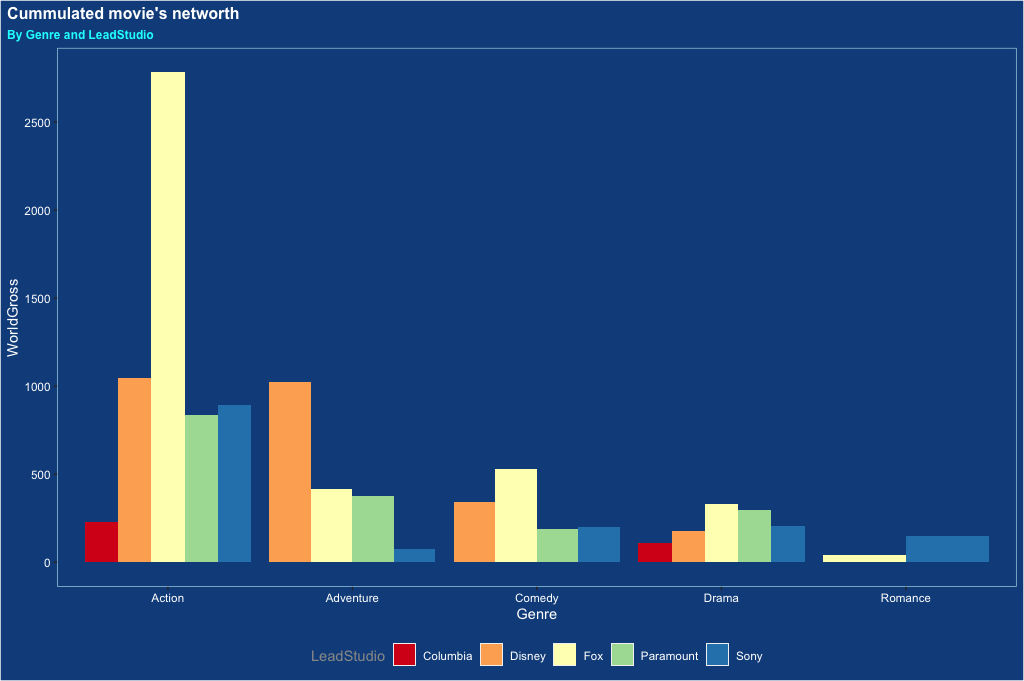
\includegraphics[width=14cm]{new/graph2.png}
\end{figure}

Entre los principales cambios que hemos realizado se encuentran el cambio del fondo a uno azul, el cambio de la paleta de colores a una más agradable, el ajuste en el título del gráfico, la adición de un subtítulo y el cambio en la posición de las etiquetas, al poner las etiquetas debajo el gráfico se vuelve más ancho, presentación más compatible cuando se usa un gráfico de barras.

\clearpage
\section{Gráfico 3 - Correlación entre BMI de varones y mujeres por país}

\begin{figure}[!h]
    \centering
    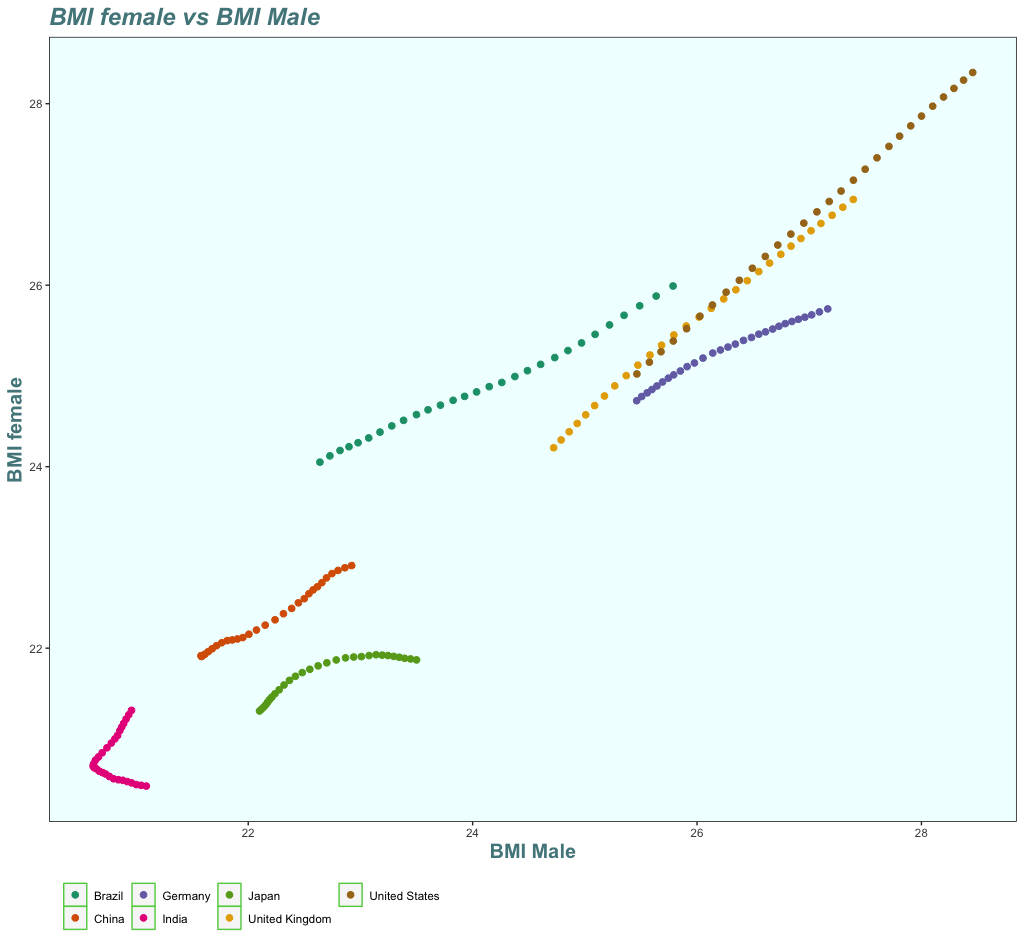
\includegraphics[width=10.5cm]{old/graph3.png}
\end{figure}

\begin{figure}[!h]
    \centering
    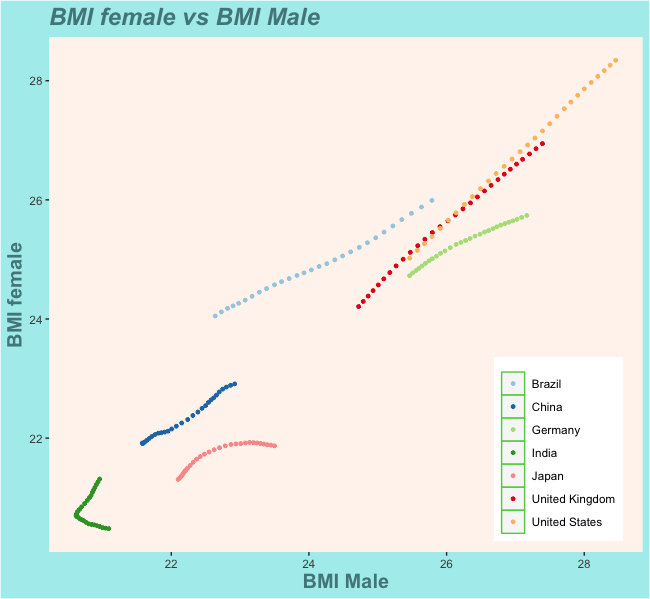
\includegraphics[width=10.5cm]{new/graph3.png}
\end{figure}

Entre los principales cambios que hemos realizado se encuentran el cambio de los colores tanto del fondo como de los puntos referentes a cada país a colores más agradables. El cambio más importante fue la inclusión del cuadro de etiquetas de cada país dentro del gráfico y no en la parte inferior, al ser un gráfico con espacios notoriamente vacios en las esquinas, la inclusión de las etiquetas en una de las esquinas aligera la lectura del gráfico.  

\end{document}
